\newpage
	\section{\Large ZIELBESTIMMUNG}
	Das Benutzungsziel ist:
	\begin{itemize}
		\item Es soll möglich sein OSM Ausschnitte über die OSM API abzufragen. Dieser Ausschnitt wird über eine Boundingbox ausgewählt.
		\item Sobald ein Ausschnitt geladen wurde, kann ein Punkt via Koordinate(Längen- und Breitengrad) ausgewählt werden und der nächstliegende Node zu diesem Punkt soll dann zentriert werden.
		\item Der Kartenausschnit soll Verschiebbar, Vergrößerbar und Verkleinerbar sein.
	\end{itemize}
	\subsection{Musskriterien}
	\begin{itemize}
		\item Das System muss auf dem Kartenbezugssystem WGS 84 laufen
		\item Das System muss nach Eingabe von Breiten- \& Längengrad eine Teilkarte ausgeben. Auf dieser Karte sind die Bundesautobahnen und Bundesstraßen sowie Richtungspfeile in die, die Autobahn/Straße verläuft, eingezeichnet. Dabei zeigen die Pfeile in die jeweilige Richtung der nächsten Node.
		\item Das System muss die Pfeile, so anpassen das die Länge der Pfeile in proportionaler abhängig zur Geschwindigkeitsbeschränkung stehen. 
		\item Das System muss nach Eingabe einer minimalen und maximalen-Eingabe eines Punkten, den Ausschnitt der Karte darstellen.
		\item Das System muss nachdem eine Karte dargestellt wurde, den ausgewählten Kartenbereich verschieben können.
		\item Das System muss nach laden eines Kartenbereichs diesen Verschieben, Vergrößern, und Verkleinern können.
	\end{itemize}
	\subsection{Abgrenzungskriterien}
	\begin{itemize}
		\item Das System ist keine Navigations Software.
	\end{itemize}
	
	
	\section{\Large PRODUKTEINSATZ}
	\subsection{Anwendungsbereiche}
	\begin{itemize}
		\item Das Produkt soll im privaten Bereich eines Benutzers Anwendung finden.\\
		Es soll nicht für gewerbliche Zwecke oder für Anbahnung von Geschäften genutzt werden.
	\end{itemize}
	\subsection{Zielgruppen}
	\begin{itemize}
		\item Die Zielgruppe sind Leute, 
		\begin{itemize}
			\item wie Herr Dr. Fünfzig
			\item die Wert auf \textbf{"Wege zur Gewinnung und Korrektur von Kartendaten"} legen.(Aus Anfordernungen des Kunden entnommen)
			\item die Initiativen für \textbf{"GeoInformation und Navigation"} unterstützen.
		\end{itemize}
	\end{itemize}
	\subsection{Betriebsbedingungen}
	\begin{itemize}
		\item Das Produkt benötigt eine stetige Internetverbindung und den Dienst der die *.OSM Dateien zur Verfügung stellt. Unser Service wird angeboten solange wir Zugriff auf die *.OSM Dateien haben.
	\end{itemize}
	
	
	\section{\Large PRODUKTÜBERSICHT}
	Gibt eine Übersicht über das Produkt, z.B. über alle wichtigen Geschäftsprozesse in Form eines Übersichtsdiagramms.
	\subsection{Usecase Diagramm}
		\begin{figure}[H]
			\centering
			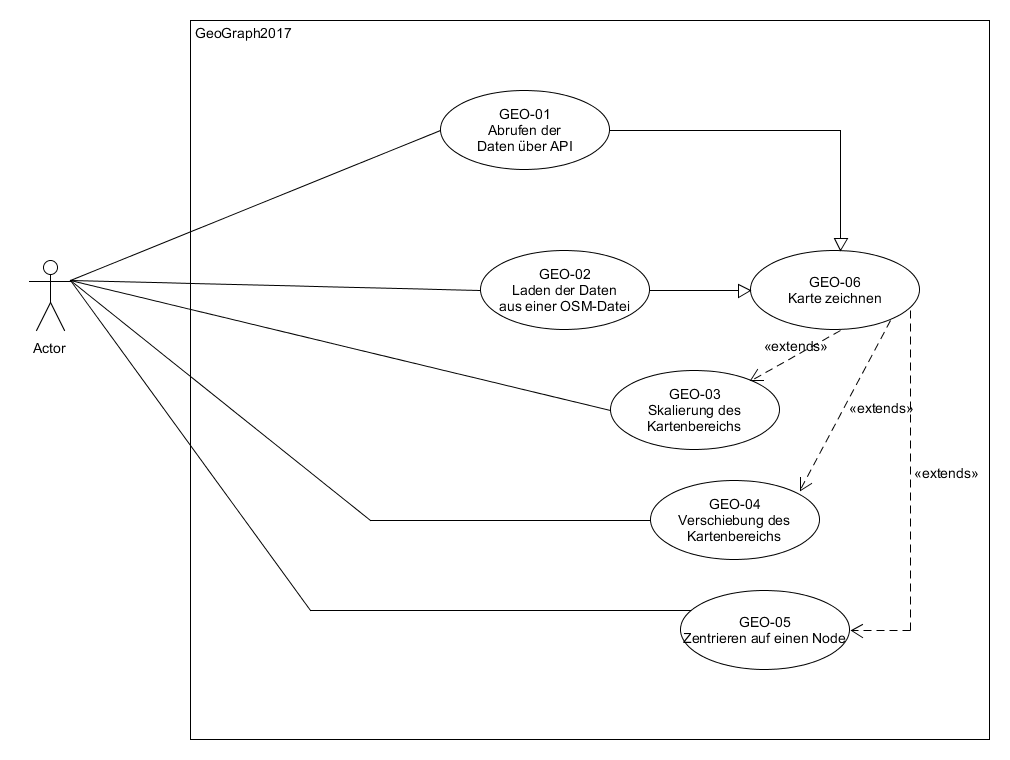
\includegraphics[width=0.7\linewidth]{images/Usecases}
			\caption{UseCase Diagramm}
			\label{fig:Usecase Diagramm}
		\end{figure}
		
		
	\section{\Large PRODUKTFUNKTIONEN}
	\subsection{Usecase-Beschreibungen}
	\begin{table}[H]
		\begin{tabular}{|p{8cm}|p{8cm}|}
			\hline
			\textbf{GEO-01 } \\ 
			\hline
			\textbf{ID :}\centering & GEO-01  \\ \hline 
			\textbf{Title :}\centering & Abruf der Daten über API \\ \hline 
			\textbf{Description :}\centering & Daten für die Karte werden per API abgerufen \\ \hline 
			\textbf{Trigger :}\centering & User klickt auf den Button "Nach Koordinaten suchen" \\ \hline 
			\textbf{Primary Actor :} \centering & User \\ \hline 
			\textbf{Preconditions :}\centering & 
			1. Programm ist gestartet \newline 
			2. User befindet sich im Reiter "Bereich" \newline
			3. User hat Boundingbox (Längengrad min/max und Breitengrad min/max) eingegeben	\\ \hline 
			\textbf{Postconditions :}\centering &  
			1. User hat den Kartenbereich erfolgreich geladen \newline 
			2. GEO-06 \\ \hline
			\textbf{Other Use Cases :}\centering & - \\ \hline  
			\textbf{Main Success Scenario :}\centering & 
			1. User gibt Boundingbox (Längen-/Breitengrad min/max) ein \newline
			2. User klickt auf "Nach Kordinaten suchen" \newline
			3. GEO-06 \\ \hline  
			\textbf{Extensions :}\centering & - \\ \hline  
			\textbf{Priority :}\centering & High \\ \hline  
		\end{tabular}
	\end{table}	
	
	\begin{table}[H]
		\begin{tabular}{|p{8cm}|p{8cm}|}
			\hline
			\textbf{GEO-02 } \\ 
			\hline
			\textbf{ID :}\centering & GEO-02  \\ \hline 
			\textbf{Title :}\centering & Laden der Daten aus einer OSM-Datei \\ \hline 
			\textbf{Description :}\centering & Daten für die Karte werden aus der hinterlegten OSM-Datei geladen \\ \hline 
			\textbf{Trigger :}\centering & User klickt auf den Button "Datei auswählen" \\ \hline 
			\textbf{Primary Actor :} \centering & User \\ \hline 
			\textbf{Preconditions :}\centering & 
			1. GEO-01 / oder OSM-Datei bereits geladen \newline
			2. User befindet sich im Reiter "Datei"\\ \hline 
			\textbf{Postconditions :}\centering & 
			1. User hat Kartenbereich aus OSM-Datei geladen \newline
			2. GEO-06 \\ \hline
			\textbf{Other Use Cases :}\centering & - \\ \hline  
			\textbf{Main Success Scenario :}\centering & 
			1. GEO-01 / oder OSM-Datei bereits vorhanden \newline
			2. User ist im Reiter "Datei" \newline
			3. User klickt auf "Datei auswählen" \newline
			4. GEO-06 \\ \hline  
			\textbf{Extensions :}\centering & - \\ \hline  
			\textbf{Priority :}\centering & High \\ \hline  
		\end{tabular}
	\end{table}
	
	\begin{table}[H]
		\begin{tabular}{|p{8cm}|p{8cm}|}
			\hline
			\textbf{GEO-03 } \\ 
			\hline
			\textbf{ID :}\centering & GEO-03  \\ \hline 
			\textbf{Title :}\centering & Skalierung des Kartenbereichs  \\ \hline 
			\textbf{Description :}\centering & Skaliert den Kartenbereich via Regler  \\ \hline 
			\textbf{Trigger :}\centering & User bewegt den Slider in den positiven/negativen Bereich  \\ \hline 
			\textbf{Primary Actor :} \centering & User \\ \hline 
			\textbf{Preconditions :}\centering & 
			1. User hat GEO-01 oder GEO-02 ausgeführt \newline
			2. User befindet sich im Reiter "Bereich"\\ \hline 
			\textbf{Postconditions :}\centering & 
			1. User bewegt Slider in den positiven/negativen Bereich \newline
			2. Kartenausschnitt vergrößert/verkleinert sich \newline
			3. GEO-06 \\ \hline
			\textbf{Other Use Cases :}\centering & - \\ \hline  
			\textbf{Main Success Scenario :}\centering & 
			1. GEO-01 oder GEO-02 \newline
			2. User ist im Reiter "Bereich" \newline
			3. User bewegt Slider in Positiven/Negativen Bereich \newline
			4. Karte wird vergrößert/verkleinert \newline
			5. GEO-06 \\ \hline  
			\textbf{Extensions :}\centering & - \\ \hline  
			\textbf{Priority :}\centering & High \\ \hline  
		\end{tabular}
	\end{table}
	
	\begin{table}[H]
		\begin{tabular}{|p{8cm}|p{8cm}|}
			\hline
			\textbf{GEO-04 } \\ 
			\hline
			\textbf{ID :}\centering & GEO-04  \\ \hline 
			\textbf{Title :}\centering & Verschiebung des Kartenbereichs \\ \hline 
			\textbf{Description :}\centering & Verschiebt den Kartenbereich via Maus \\ \hline 
			\textbf{Trigger :}\centering & User bewegt die Maus in den Kartenausschnitt und hält die linke Maustaste gedrückt und schiebt dann in x/y Richtung  \\ \hline 
			\textbf{Primary Actor :} \centering & User \\ \hline 
			\textbf{Preconditions :}\centering & 
			1. GEO-01 oder GEO-02 \newline 
			2. User befindet sich im Reiter "Bereich"\\ \hline 
			\textbf{Postconditions :}\centering & 
			1. User bewegt die Maus in x/y Richtung \newline
			2. Der Kartenausschnitt bewegt sich in x/y Richtung \newline
			3. GEO-06 \\ \hline
			\textbf{Other Use Cases :}\centering & - \\ \hline  
			\textbf{Main Success Scenario :}\centering & 
			1. GEO-01 oder GEO-02 \newline
			2. User ist im Reiter "Bereich" \newline
			3. User hält Maus gedrückt und schiebt den Kartenausschnitt \newline
			4. GEO-06 \\ \hline  
			\textbf{Extensions :}\centering & 
			1. Nur zuvor geladener Kartenausschnitt wird angezeigt \\ \hline  
			\textbf{Priority :}\centering & High \\ \hline  
		\end{tabular}
	\end{table}
	
	\begin{table}[H]
		\begin{tabular}{|p{8cm}|p{8cm}|}
			\hline
			\textbf{GEO-05 } \\ 
			\hline
			\textbf{ID :}\centering & GEO-05  \\ \hline 
			\textbf{Title :}\centering & Nächsten Punkt suchen und Ansicht auf Node zentrieren \\ \hline 
			\textbf{Description :}\centering & Zentrierung auf einer Node nach Eingabe von Langen-und Breitengrad \\ \hline 
			\textbf{Trigger :}\centering & User gibt Breiten-und Längengrad ein und die nächstgelegende Node wird zentriert \\ \hline 
			\textbf{Primary Actor :} \centering & User \\ \hline 
			\textbf{Preconditions :}\centering & 
			1. GEO-01 oder GEO-02 \newline 
			2. User befindet sich im Reiter "Bereich" \\ \hline 
			\textbf{Postconditions :}\centering &
			1. Kartenausschnitt wird auf die nächstgelgende Node verschoben \newline
			2. Karte wird auf die Node zentriert \newline
			3. GEO-06 \\ \hline
			\textbf{Other Use Cases :}\centering & - \\ \hline  
			\textbf{Main Success Scenario :}\centering &
			1. GEO-01 oder GEO-02 \newline
			2. User ist im Reiter "Bereich" \newline
			2. Kartenausschnitt wird verschoben \newline
			3. Karte wird auf Node zentriert \newline
			4. GEO-06 \\ \hline  
			\textbf{Extensions :}\centering & - \\ \hline  
			\textbf{Priority :}\centering & High \\ \hline  
		\end{tabular}
	\end{table}	
	
	\begin{table}[H]
		\begin{tabular}{|p{8cm}|p{8cm}|}
			\hline
			\textbf{GEO-06 } \\ 
			\hline
			\textbf{ID :}\centering & GEO-06  \\ \hline 
			\textbf{Title :}\centering & Karte zeichnen \\ \hline 
			\textbf{Description :}\centering & Karte zeichen nach Eingabe von Boundingbox (Längen-/Breitengrad min/max) \\ \hline 
			\textbf{Trigger :}\centering & User gibt Boundingbox (Längengrad min/max und Breitengrad min/max) ein und die Karte wird gezeichnet \\ \hline 
			\textbf{Primary Actor :} \centering & User \\ \hline 
			\textbf{Preconditions :}\centering & User befindet sich im Reiter "Bereich" \\ \hline 
			\textbf{Postconditions :}\centering	& 
			1. GEO-01 oder GEO-02 \\ \hline		
			\textbf{Other Use Cases :}\centering & - \\ \hline  
			\textbf{Main Success Scenario :}\centering &
			1. GEO-01 oder GEO-02 \newline
			2. Karte wird gezeichnet \\ \hline  
			\textbf{Extensions :}\centering & - \\ \hline  
			\textbf{Priority :}\centering & High \\ \hline  
		\end{tabular}
	\end{table}			
	
	\subsection{Aktivitätsdiagramm}
		\begin{figure}[H]
			\centering
			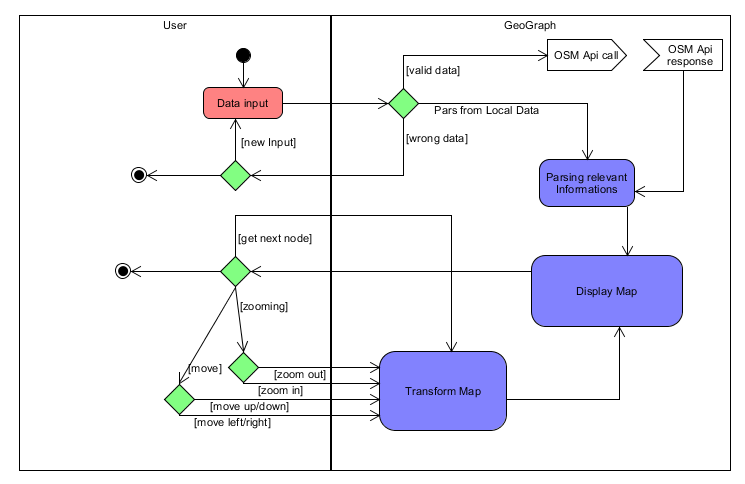
\includegraphics[width=0.7\linewidth]{images/Ablauf}
			\caption{Aktivitäts Diagramm}
			\label{fig:Aktivitäts Diagramm}
		\end{figure}
	\subsection{Sequenzdiagramm}
	\begin{figure}[H]
	\centering
	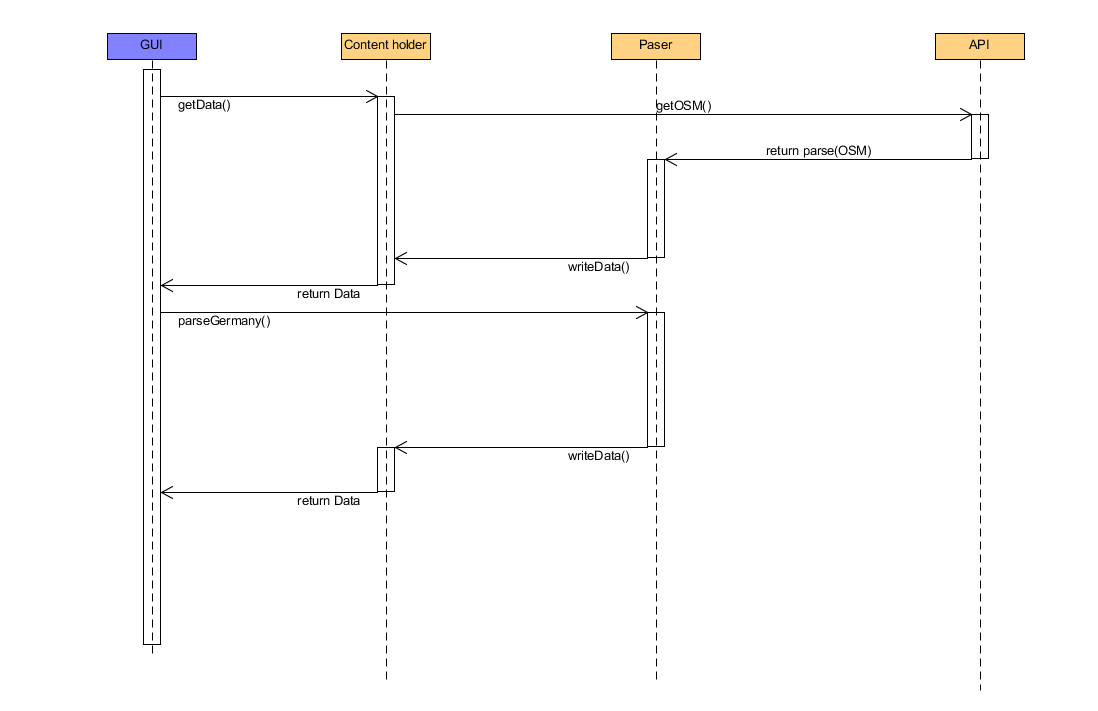
\includegraphics[width=0.7\linewidth]{images/Squenz}
	\caption{Sequenz Diagramm}
	\label{fig:Sequenz Diagramm}
	\end{figure}
	
\newpage
	\section{\Large PRODUKTDATEN}
		Langfristig sollen folgende Daten im System gespeichert | ausgelesen werden:
	\begin{itemize}
		\item Speicherung der OSM-Datei in folgendem Format: 
		\begin{itemize}
			\item Min und Max der BoundingBox
			\item 51.9\_52.1\_52.1\_53.0.osm (Beispiel)
		\end{itemize}
		\item Laden der Daten via Overpass API
	\end{itemize}
	\subsection{Analyseklassendiagramm}	
		\begin{figure}[H]
		\centering
		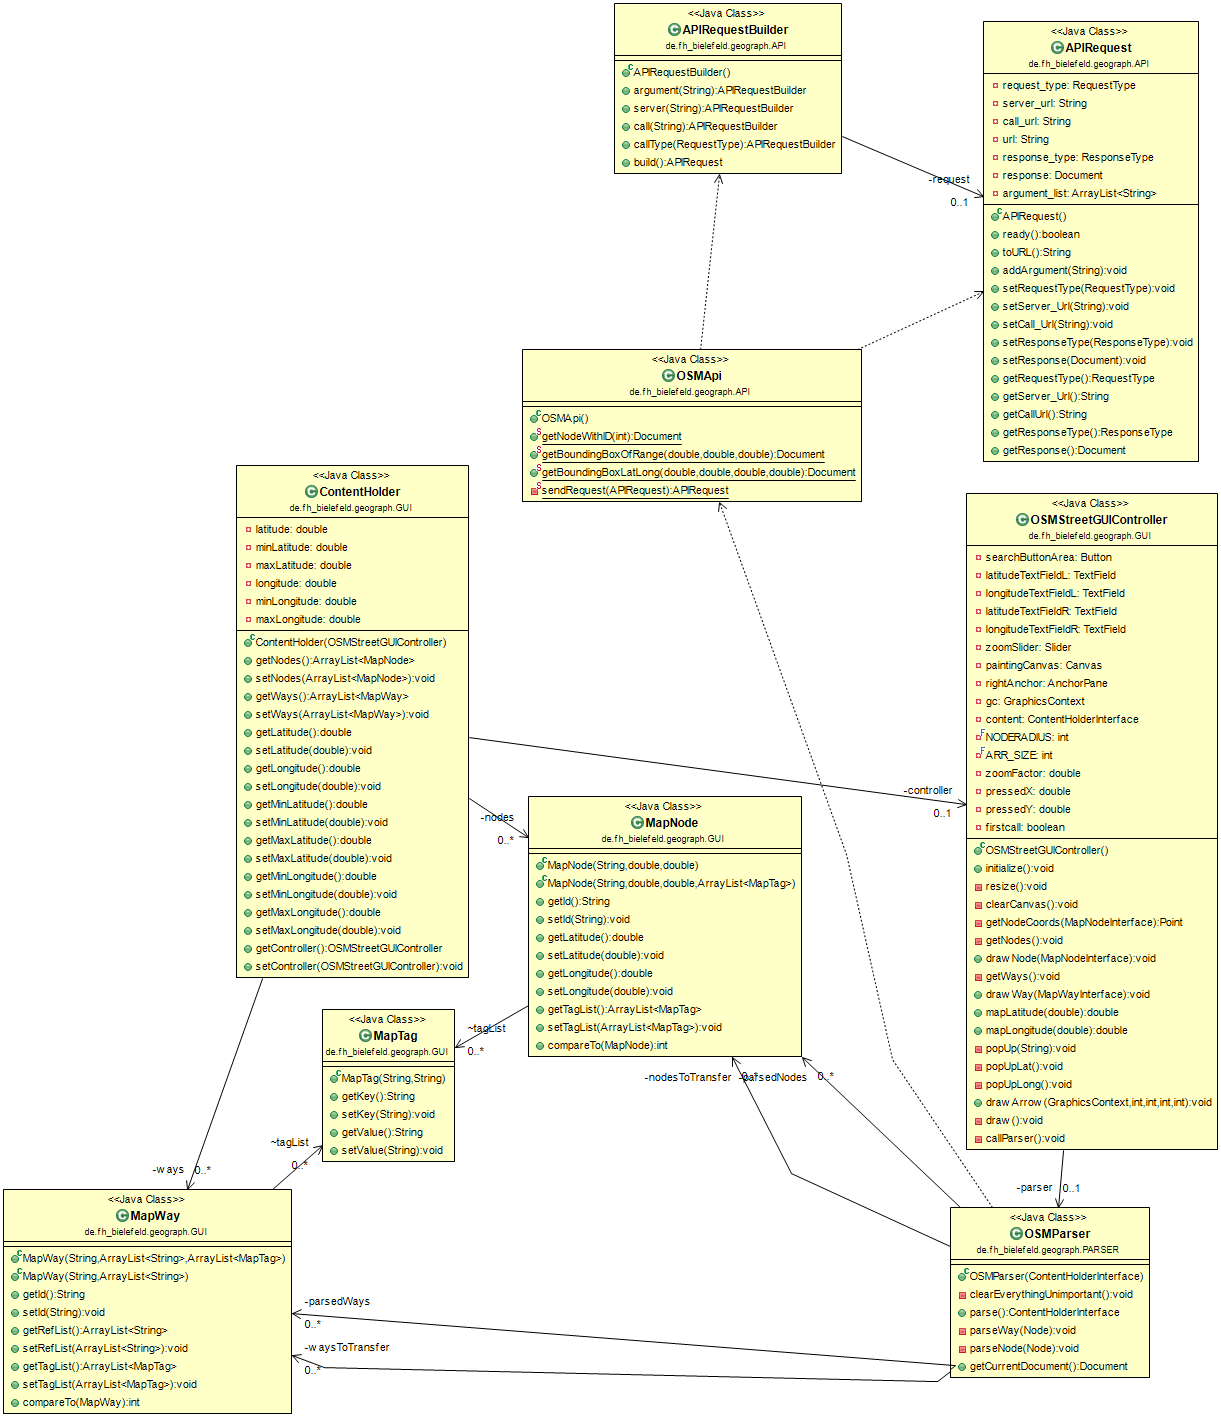
\includegraphics[width=0.7\linewidth]{images/Klassendiagramm_v2}
		\caption{Klassendiagramm}
		\label{fig:Klassendiagramm}
	\end{figure}
	\subsection{Paketdiagramm}
		\begin{figure}[H]
			\centering
			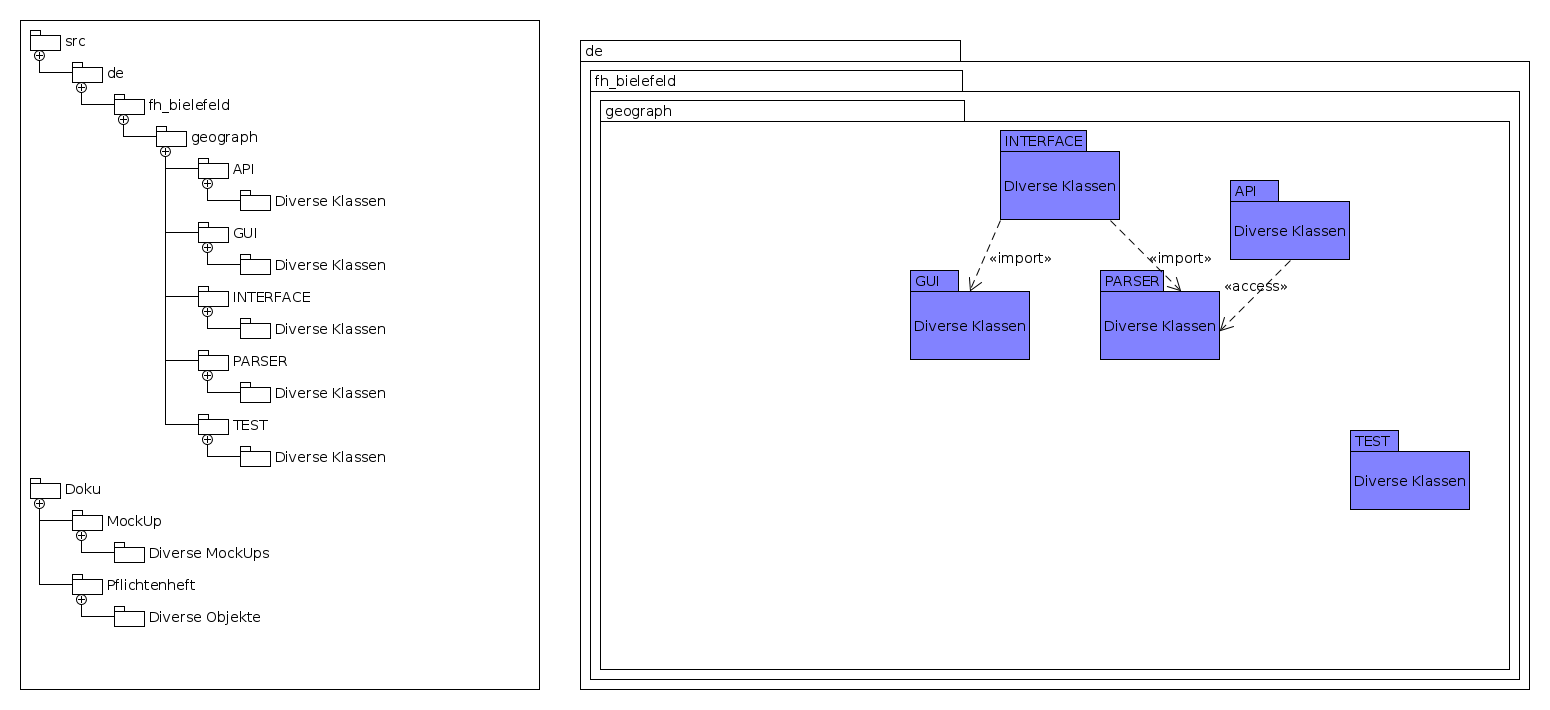
\includegraphics[width=0.7\linewidth]{images/Paketdiagramm}
			\caption{Paketdiagramm}
			\label{fig:Paketdiagramm}
		\end{figure}
	\subsection{Domänenklassendiagramm}
		\begin{figure}[H]
			\centering
			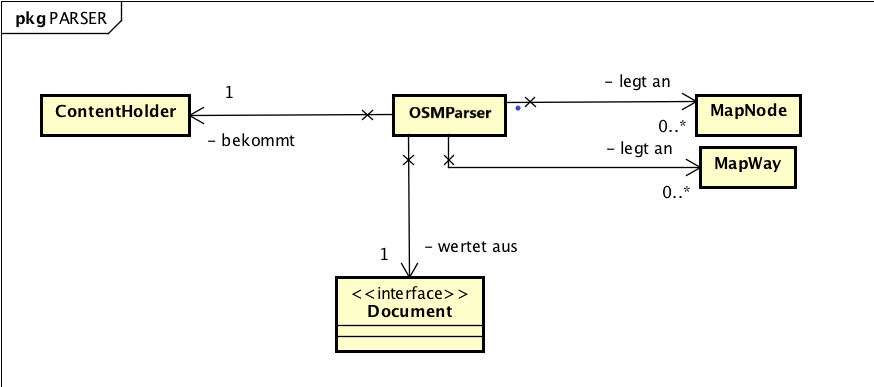
\includegraphics[width=0.7\linewidth]{images/DomaenenKlassendiagramm_v3}
			\caption{Domänenklassendiagramm}
			\label{fig:Domänenklassendiagramm}
		\end{figure}
	\section{\Large PRODUKTLEISTUNGEN}
	\begin{itemize}
		\item Nicht genauer spezifiziert.
	\end{itemize} 
		
	\section{\Large QUALITÄTSANFORDERUNGEN}
	\begin{itemize}
		\item Nicht genauer spezifiziert.
	\end{itemize}
	
	\section{\Large BENUTZEROBERFLÄCHE}
	Es gibt eine Rolle und das ist die des Users der das Prgoramm ausführt (GUI).
	\begin{figure}[H]
	\centering
	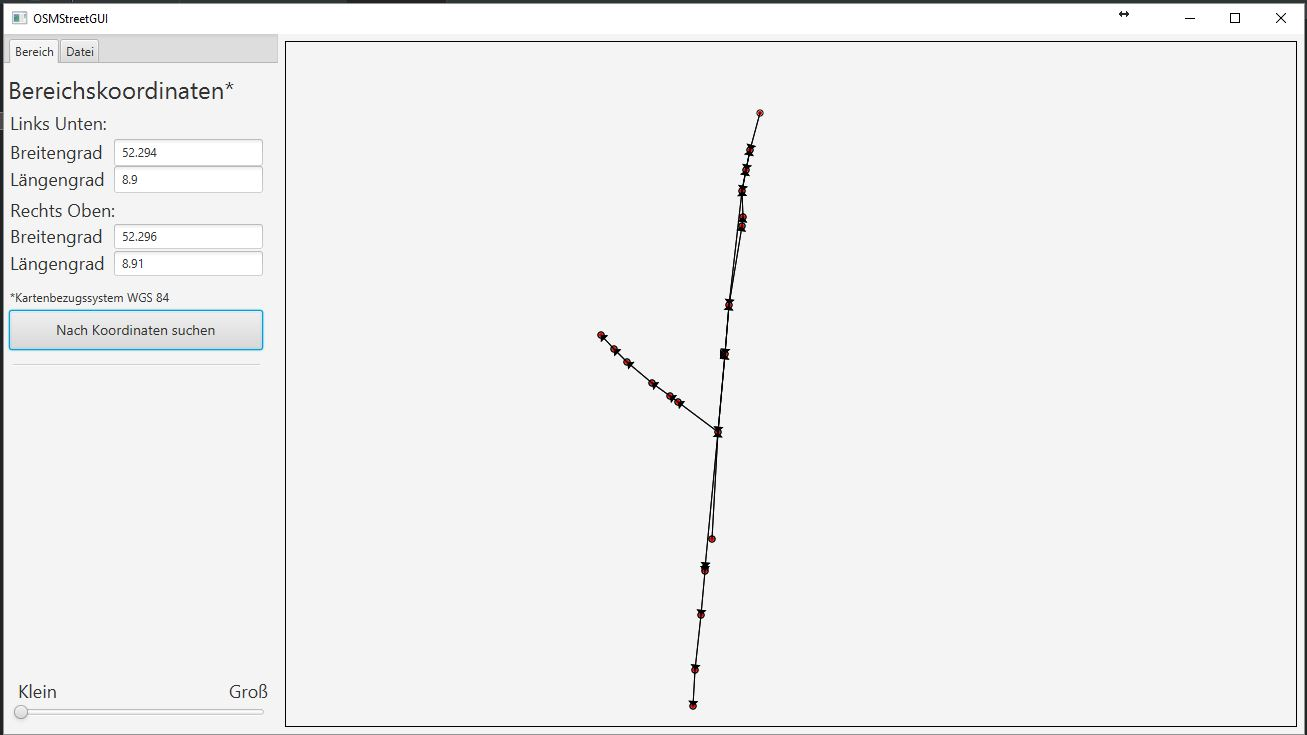
\includegraphics[width=0.7\linewidth]{images/BereichReiter}
	\caption{Benutzeroberfläche im Reiter Bereich}
	\label{fig:GUI}
	\end{figure}
	
	\begin{figure}[H]
	\centering
	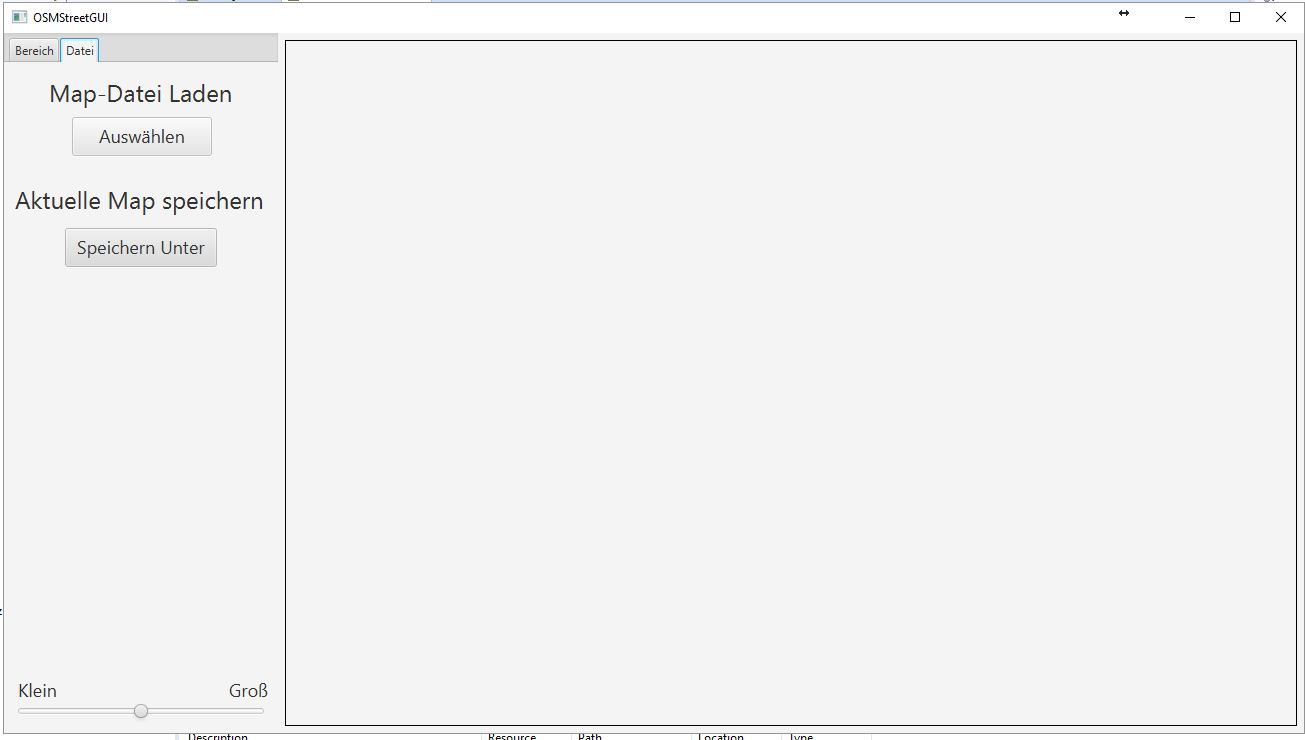
\includegraphics[width=0.7\linewidth]{images/DateiReiter}
	\caption{Benutzeroberfläche im Reiter Datei}
	\label{fig:GUI2}
	\end{figure}
	
	\subsection{Zustandsdiagramme}
	\begin{figure}[H]
	\centering
	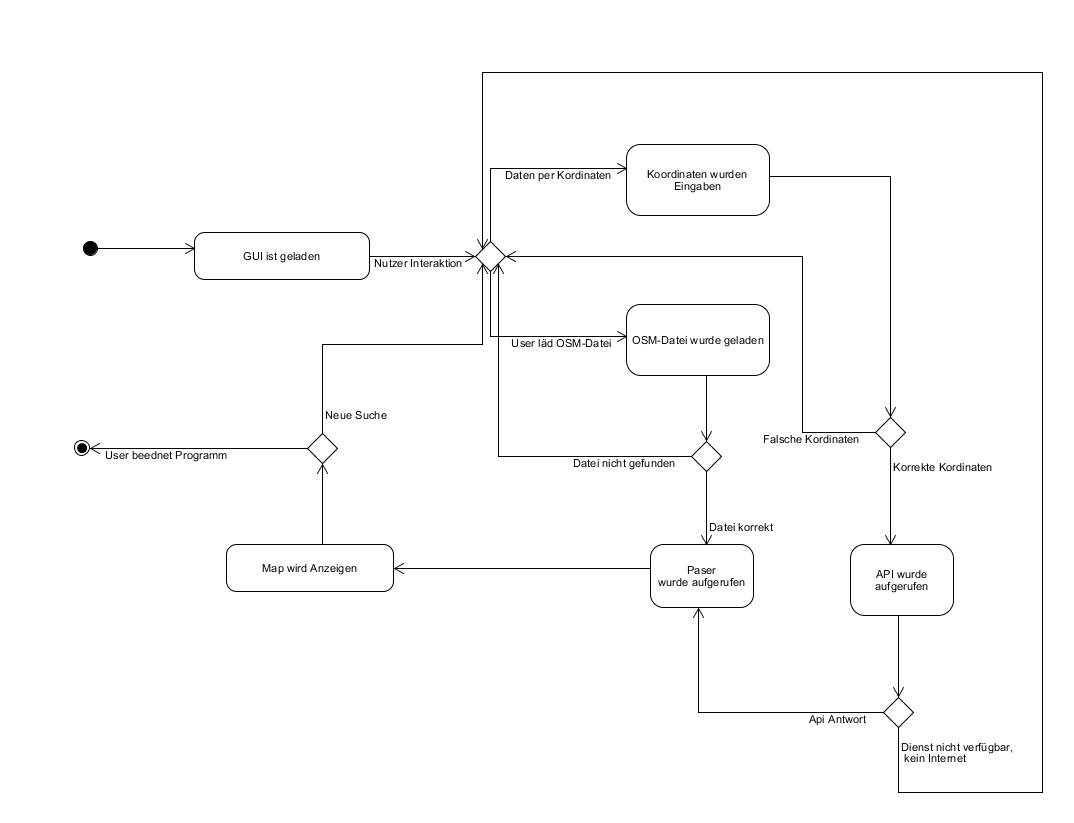
\includegraphics[width=0.7\linewidth]{images/Zustandsdiagramm}
	\caption{Zustands Diagramm}
	\label{fig:Zustands Diagramm}
	\end{figure}
	
	\section{\Large NICHTFUNKTIONALE ANFORDERUNGEN}
	Es werden alle Anforderungen aufgeführt, die sich nicht auf die Funktionalität, \textbf{ die Leistung} und \textbf{ die Benutzungsoberfläche} beziehen, z.B. :
	\begin{itemize}
		\item Einzuhaltende \textbf{Gesetze}
		\item Einzuhaltende \textbf{Normen}
		\item Testat durch externe Prüfungsgesellschaft
		Revisionsfähigkeit 
		\item Ordnungsmäßigkeit der Buchführung
		\item \textbf{ Sicherheitsanforderungen, z.B. :}
		\begin{itemize}
			\item Richtigkeit der Nodes
			\item Richtigkeit der Pfeile
			\item Genaues Darstellen der Nodes in Abhängigkeit zur OSM-Datei
			\item Genauigkeit der BoundingBox
			\item Genauigkeit beim Skalieren
		\end{itemize}  
		\item Plattformabhängigkeiten
		\item Performant in Abhängigkeit zur Downloadgeschwindigkeit und API
		\item Wenn der markierte Bereich der Boundingbox zu groß gewählt wurde (range > 0,25), dann kann das laden der Nodes sehr lange dauern
		\item Aktuelle Betriebssysteme abdecken(Windows, Linux)
		\item Abgefragte OSM-Datein werden lokal gespeichert mit den Min und Max Angaben der BoundingBox	(bsp. 51.9\_52.1\_52.1\_53.0.osm) 
	\end{itemize} 

	
	\section{\Large TECHNISCHE PRODUKTUMGEBUNG}
   	In diesem Kapitel wird die technische Umgebung des Produkts beschrieben.\\
   	Bei Client / Server-Anwendungen ist die Umgebung jeweils für Clients und Server getrennt anzugeben.
	\subsection{Software}
	\begin{itemize}
		\item Erfordert \textbf{Java 8.x} auf dem Client
		\begin{itemize}
			\item getestet und entworfen wird für :
			\begin{itemize}
				\item PC | Laptop
				\begin{itemize}
					\item Windows ab Version 7
					\item Linux
				\end{itemize}
			\end{itemize}
		\end{itemize}
	\end{itemize}
	\subsection{Hardware}
	\begin{itemize}
		\item \textbf{Internetfähiges Gerät :}
		\begin{itemize}
			\item PC | Laptop
			\item \textbf{Minimale Bildschirmauflösung :}
				\begin{itemize}
					\item 1024 x 768 Pixel Hochformat / Querformat
				\end{itemize}
					\item \textbf{Maximale Bildschirmauflösung :}
				\begin{itemize}
				\item 4096 × 2160 Pixel Hochformat / Querformat
				\end{itemize}		
		\end{itemize}
	\end{itemize}
	\subsection{Orgware}
	\begin{itemize}
		\item Der Client benötigt eine Internetverbindung.
		\item Um eine befriedigende Nutzererfahrung zu gewährleisten, werden folgende Bandbreiten-Untergrenzen definiert:
		\begin{itemize}
			\item \textbf{ PC | Laptop :}
			\begin{itemize}
				\item DSL Verbindung mit min. 2 Mbit/s Download-Bandbreite
			\end{itemize}
		\end{itemize}
	\end{itemize}	
	\subsection{Produkt-Schnittstellen}
	\begin{itemize}
		\item \textbf{OSM API}-Schnittstelle
		\begin{itemize}
			\item Anfragen in einem auf \textbf{REST} basierten Muster
			\item Übertragen der Daten mittels des \textbf{HTTP} Protokolls
			\item \textbf{2 Zugriffspunkte :}
			\begin{itemize}
				\item \textbf{OpenStreetMap} V06 API \href{http://wiki.openstreetmap.org/wiki/API_v0.6}{OpenStreetMap Wiki}
				\item \textbf{Overpass} API \href{http://overpass-api.de/}{Overpass API Hauptseite}
			\end{itemize}
			\item \textbf{API Nutzung :}
			\begin{itemize}
				\item Wir benutzen zwei API's :
				\begin{itemize}
					\item um das System vor Ausfällen zu schützen
					\item falls ein Dienst die Arbeit einstellt z.B.(OpenStreetMap V06 API), ist unser Programm weiterhin benutzbar, da wir auf andere API's ausweichen können
				\end{itemize}  
			\end{itemize}
			\item \textbf{2 Operationen :}
			\begin{itemize}
				\item \textbf{GetNodeByID} Weitere Informationen zu einer bestimmten Node abfragen
				\item \textbf{BoundingBox} Alle \textit{Relations}, \textit{Ways} und \textit{Nodes} ein einem
					bestimmten Bereich abfragen
			\end{itemize}
			\item \textbf{Anfragen, Ablageverzeichnis und Namenskonvention :}			
			\begin{itemize}
				\item Erfolgreich ausgeführte Anfragen werden Lokal abgelegt
				\item Ablageverzeichnis relativ zum Projektpfad unter \textit{requests}
			\end{itemize}
				\item \textbf{Namenskonvention im Format :}
				\begin{itemize}
				\item ABFRAGETYP\_\_ABFRAGENPARAMETER\_\_\\ABFRAGEZEITPUNKT.osm
				\end{itemize}		
				GENAUER					
		\end{itemize}
	\end{itemize}
	
	\section{\Large SPEZIELLE ANFORDERUNGEN AN DIE ENTWICKLUNGS-UMGEBUNG}
	Entwicklung- und Testumgebung des Frontends: Siehe 10 Technische Produktentwicklung 
	\subsection{Software}
	\subsection{Hardware}
	\subsection{Orgware}
	\subsection{Entwicklungsschnittstellen}
	
	
	\section{\Large GLIEDERUNG IN TEILPRODUKTE}
	
	
	\section{\Large ERGÄNZUNGEN}
	Ein erster Testbetrieb wird in der Arbeitsumgebung des Kunden stattfinden. Dort wird dann zunächst ausgiebig die Stabilität und Sicherheit des Systems getestet.
	
\newpage
	\section{\Large GLOSSAR}
	In diesem Kapitel wird die spezifische Sprache des Auftraggebers wie \textbf{ Kürzel } und \textbf{ Fachbegriffe } beschrieben, z.B. :
	\begin{itemize}
		\item \textbf{ User }
		\begin{itemize}
			\item Der User ist der Benutzer des Programms.
		\end{itemize}
		\item \textbf{ Pfeile }
		\begin{itemize}
			\item Ein Pfeil zeigt in Richtung des nächsten Nodes auf der Straße, seine Länge ist abhängig zur Skalierung und der Geschwindigkeitsbeschränkung.
		\end{itemize}
		\item \textbf{ BoundingBox }
		\begin{itemize}
			\item Eine BoundingBox ist ein Ausschnitt eines Kartenbereichs, die Grenzen des Ausschnittes werden von einem minimal Wert bestehend aus Längen- und Breitengrad bestimmt, und einem maximal Wert ebenfalls aus Längen- und Breitengrad abgegenzt. 
		\end{itemize}
		\item \textbf{ Node }
		\begin{itemize}
			\item Ein Node stellt einen Punkt einer Straße auf der Karte dar, mehrere Nodes bilden somit einen Straßenverlauf ab
		\end{itemize}
		\item \textbf{ OSM-Datei }
		\begin{itemize}
			\item Eine OSM-Datei beinhalten die Karteninformationen im XML Format, in diesem XML Format werden die Nodes aufgelistet. 
		\end{itemize}
		\item \textbf{ Java }
		\begin{itemize}
			\item Java ist eine Plattform unabhängige Programmiersprache, in der der GeoGraph2017 umgesetzt wird.
		\end{itemize}
		\item \textbf{ API }
		\begin{itemize}
			\item Eine Programmierschnittstelle, genauer Schnittstelle zur Anwendungsprogrammierung(englisch: application programming interface), ist ein Programmteil, der von einem Softwaresystem anderen Programmen zur Anbindung an das System zur Verfügung gestellt wird. 
		\end{itemize}
	\end{itemize}

		